\documentclass[11pt]{article}

\author{Math 123}
\date{Due March 12, 2021 by 5pm} 
\title{Homework 6}

\usepackage{graphicx,xypic}
\usepackage{amsthm}
\usepackage{amsmath,amssymb}
\usepackage{amsfonts}
\usepackage{xcolor}
\usepackage[margin=1in]{geometry}
\usepackage[shortlabels]{enumitem}
\newtheorem{problem}{Problem}
\renewcommand*{\proofname}{{\color{blue}Solution}}


\usepackage{fancyhdr}
\pagestyle{fancy}
\rhead{Math 123, Homework 6}

\setlength{\parindent}{0pt}
\setlength{\parskip}{1.25ex}


\begin{document}

\maketitle

% You are required to put your name here:
{\bf\Large Name:} 


\vspace{.3in}
Topics covered: vertex cuts, connectivity, Menger's theorem, network flows, coloring

Instructions: 
\begin{itemize}
\item This assignment must be submitted on Gradescope by the due date. 
\item If you collaborate with other students (which is encouraged!), please mention this near the corresponding problems. 
\item Some problems from this assignment come from West's book, as indicated next to the problem. In some cases, the statements on this assignment differ slightly from the book. 
\item If you are stuck please ask for help (from me or your classmates). Occasionally problems may require ingredients not discussed in the course. 
\item You may freely use any fact proved in class. In general, you should provide proof for facts used that were not proved in class. 
\end{itemize}

\pagebreak 


\begin{problem}
Let $G$ be a graph. 
\begin{enumerate}[(a)]
\item Give a counterexample to the following statement: If $G$ has an edge such that $G\setminus e$ is disconnected, then $G$ has a one-vertex vertex cut. 
\item Add a hypothesis to correct the above statement. 
\end{enumerate} 
\end{problem}

\begin{proof}

\end{proof}

\pagebreak

\begin{problem}
Compute (with proof) $\kappa(u,v)$ for the graph below.
\begin{center}
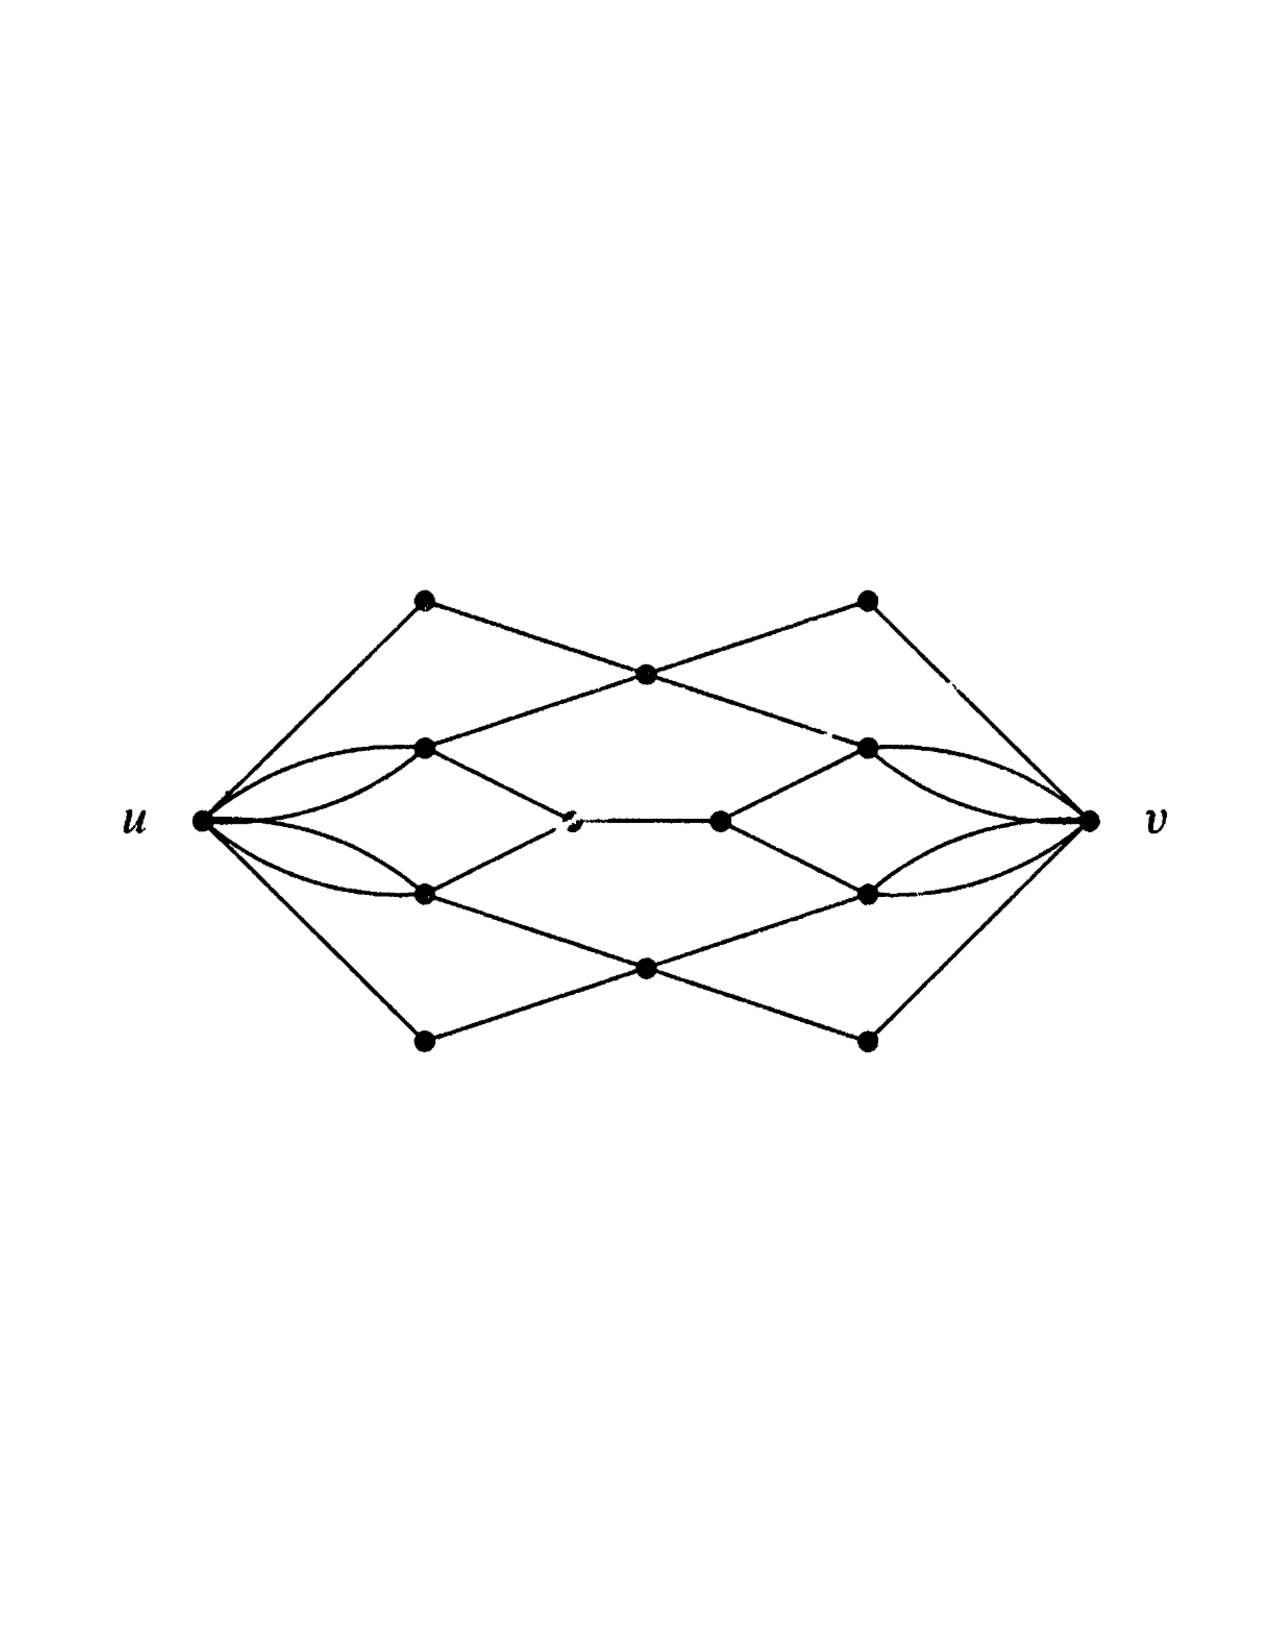
\includegraphics[scale=.4]{hw6-graph.pdf}
\end{center}
\end{problem}

\begin{proof}

\end{proof}

\pagebreak

\begin{problem}
Find (with proof) the smallest $3$-regular graph having connectivity $1$. \footnote{Hint: consider a 1-element vertex cut $S$. What does $G\setminus S$ look like? } 
\end{problem}

\begin{proof}

\end{proof} 

\pagebreak

\begin{problem}
Fix $k\ge2$. Prove that the hypercube $Q_k$ is $k$-connected by constructing $k$ pairwise internally disjoint $x,y$-paths for each pair of vertices $x,y$. 
\end{problem}

\begin{proof}

\end{proof}

\pagebreak

\begin{problem}
Use network flows to prove K\"onig's theorem. \footnote{Hint: form a network from the bipartite graph.. (How exactly?) Be sure to give plenty of details.} 
\end{problem}

\begin{proof}

\end{proof}

\pagebreak


\begin{problem}
Prove that every graph $G$ has a vertex ordering relative to which the greedy coloring uses $\chi(G)$ colors. 
\end{problem}

\begin{proof}

\end{proof}

\pagebreak

\begin{problem}
For a graph $G$, let $G'$ be the graph obtained by the Mycielski construction. Show that if $G$ is critical, then $G'$ is also critical. \footnote{Hint: it may help to work through this concretely for the Gr\"otzsch graph.}
\footnote{Show $\chi(G'\setminus e)<\chi(G')$ by cases. The trickiest case is $e=\{v_i,u_j\}$. One way to approach this is to start by coloring $H'$ with $H\subset G\setminus e'$, where $e'=\{v_i,v_j\}$...}
\end{problem}

\begin{proof}

\end{proof}



\end{document}